\begin{slide}{Example: Graph Colouring (Instance)}

\begin{minipage}{0.4\textwidth}
\includegraphics[width=7cm]{536970904.Dot.eps}
\end{minipage}%
\begin{minipage}{0.5\textwidth}
\begin{small}
\begin{verbatim}
Give a conflict-free node colouring of
Graph { knoten = mkSet [ 1 , 2 , 3 , 4 , 5 , 6 , 7 , 8 , 9 , 10 ]
  , kanten = mkSet [ kante 1 6 , kante 1 7 , kante 1 9 , kante 2 5
     , kante 2 7 , kante 2 8 , kante 2 9 , kante 3 6 , kante 3 7
     , kante 3 8 , kante 3 9 , kante 4 5 , kante 4 6 , kante 4 7
     , kante 5 6 , kante 5 10 , kante 6 7 , kante 6 8 , kante 6 10
     , kante 8 9 , kante 8 10 , kante 9 10 
     ] 
  }
with at most 3 different colours.
\end{verbatim}
\end{small}  
\end{minipage}

\end{slide}

\begin{slide}{Example: Graph Colouring (Solution)}
Input
\begin{small}
\begin{verbatim}
listToFM [ ( 1 , C ) , ( 2 , C ) , ( 3 , B ) , ( 4 , B ) , ( 5 , B )
    , ( 6 , A ) , ( 7 , A ) , ( 8 , C ) , ( 9 , C ) , ( 10 , C ) 
\end{verbatim}
\end{small}
Grading:
\begin{small}
\begin{verbatim}
is the set
    nodes of graph =
    mkSet [ 1 , 2 , 3 , 4 , 5 , 6 , 7 , 8 , 9 , 10 ]
a subset of the set
    coloured nodes = mkSet [ 1 , 2 , 3 , 4 , 5 , 6 , 7 , 8 , 9 , 10 ]
? Yes.
These edges connect nodes of equal colour:
    [ kante 1 9 , kante 2 8 , kante 2 9 , kante 4 5 , kante 6 7
    , kante 8 9 , kante 8 10 , kante 9 10 ]
\end{verbatim}
\end{small}

\end{slide}

\begin{slide}{Typische Anwendung}

Problem (Bsp: 3SAT)
\begin{itemize}
\item Instanz: eine Formel in 3-KNF
\item L�sung: eine erf�llende Belegung
\end{itemize}

Ablauf mit \autotool\ :
\begin{itemize}
\item Tutor konfiguriert Generator
\item \autotool\ w�rfelt Instanz
  (f�r jeden Studenten eine andere)
\item Student gibt (vermutete) L�sung ein
\item \autotool\ verifiziert L�sung,
  gibt ausf�hrlichen Bericht (sofort)
\end{itemize}

\end{slide}




\begin{slide}{Example: Graph Colouring (Configuration)}

the tutor did choose this:
\begin{itemize}
\item semantics:

problem type: \verb|Col-Quiz| and parameters for generator
\begin{verbatim}
Config { nodes = 10 , edges = 30 , chi = 3 }
\end{verbatim}
\item bookkeeping:

school, lecture, exercise, time span, rating (level)
\end{itemize}

\end{slide}
